% Copyright 2016 by Wang Kunzhen <wangkunzhen1993@gmail.com>.
%
% This is a latex template adapted from Till Tantau's Beamer template.
% It adds theme customizations for the convenience of users from the
% National University of Singapore. 
% 
% In principle, this file can be redistributed and/or modified under
% the terms of the GNU Public License, version 2.
%
% However, this file is supposed to be a template to be modified
% for your own needs. For this reason, if you use this file as a
% template and not specifically distribute it as part of a another
% package/program, I grant the extra permission to freely copy and
% modify this file as you see fit and even to delete this copyright
% notice. 

\documentclass[xcolor=dvipsnames]{beamer}

\newcommand{\Ch}{\mathit{Ch}}
\newcommand{\ch}{\mathit{ch}}
\newcommand{\Av}{\mathit{Av}}
\newcommand{\av}{\mathit{av}}
\newcommand{\CC}{\mathit{CC}}
\newcommand{\SCC}{\mathit{SCC}}
\newcommand{\core}{\mathit{Core}}
\newcommand{\I}{\mathit{I}}
\newcommand{\VI}{\mathit{VI}}
\newcommand{\AMI}{\mathit{AMI}}

% There are many different themes available for Beamer. A comprehensive
% list with examples is given here:
% http://deic.uab.es/~iblanes/beamer_gallery/index_by_theme.html
% You can uncomment the themes below if you would like to use a different
% one:
%\usetheme{AnnArbor}
%\usetheme{Antibes}
%\usetheme{Bergen}
% \usetheme{Berkeley}
%\usetheme{Berlin}
%\usetheme{Boadilla}
% \usetheme{boxes}
%\usetheme{CambridgeUS}
%\usetheme{Copenhagen}
%\usetheme{Darmstadt}
\usetheme{default}
%\usetheme{Frankfurt}
%\usetheme{Goettingen}
%\usetheme{Hannover}
% \usetheme{Ilmenau}
% \usetheme{JuanLesPins}
% \usetheme{Luebeck}
% \usetheme{Madrid}
% \usetheme{Malmoe}
%\usetheme{Marburg}
% \usetheme{Montpellier}
% \usetheme{PaloAlto}
% \usetheme{Pittsburgh}
% \usetheme{Rochester}
% \usetheme{Singapore}
% \usetheme{Szeged}
% \usetheme{Warsaw}

\usecolortheme{seagull}

\definecolor{nus-orange}{RGB}{239,124,0} 
\definecolor{nus-white}{RGB}{255,255,255}
\definecolor{nus-blue}{RGB}{0,61,124}
\definecolor{nus-black}{RGB}{0,0,0}

% Uncomment this section if you want the title background for each slide to be gradient like decaying from nus-orange to nus-white.
% \useoutertheme{shadow}
% \usepackage{tikz}
% \usetikzlibrary{shadings}
% \colorlet{titleleft}{nus-orange}
% \colorlet{titleright}{nus-orange!45!nus-white}
% \makeatletter
% \pgfdeclarehorizontalshading[titleleft,titleright]{beamer@frametitleshade}{\paperheight}{%
%   color(0pt)=(titleleft);
%   color(\paperwidth)=(titleright)}
% \makeatother
% End of gradient slide title effect.

% \setbeamercolor{section in head/foot}{bg=nus-blue, fg=nus-white}
% \setbeamercolor{subsection in head/foot}{bg=nus-blue, fg=nus-white}
% \setbeamercolor{frametitle}{bg=nus-orange, fg=nus-black}
% \setbeamercolor{title}{bg=nus-orange, fg=nus-white}
% \setbeamercolor{alerted text}{fg=nus-orange}
% \setbeamercolor{block title}{fg=nus-blue}
% \setbeamercolor{block body}{fg=nus-black}

\setbeamertemplate{theorems}[numbered]
\setbeamertemplate{propositions}[numbered]

\setbeamertemplate{bibliography item}{\insertbiblabel}

\setbeamertemplate{title page}[default][colsep=-4bp,rounded=true, shadow=true]

\title{Learning Cooperative Solution Concepts From Voting Behavior}

\subtitle{A Case Study on the Israeli Parliament}

\author{Lu Wei}

\institute[National University of Singapore] % (optional, but mostly needed)
{
  Department of Computer Science\\
  National University of Singapore
}

\titlegraphic{
   \includegraphics[width=2cm]{nus-logo}
}

\date{Jan 2020}

% Uncomment this, if you want the table of contents to pop up at
% the beginning of each subsection:
% \AtBeginSubsection[]
% {
%   \begin{frame}<beamer>{Outline}
%     \tableofcontents[currentsection,currentsubsection]
%   \end{frame}
% }

\begin{document}

\begin{frame}
  \titlepage
\end{frame}

\begin{frame}{Outline}
  \tableofcontents
\end{frame}

\section{Introduction}

\begin{frame}{Background}
  \begin{itemize}
    \item Coalition formation games:
    \begin{itemize}
      \item Mostly theoretical analysis
      \item Most models require full information on player preference
      \item Lack of large dataset with ground truth
    \end{itemize}
    \item Clustering \& community detection:
    \begin{itemize}
      \item Data-driven analysis
      \item Missing strategic behavior modelling
    \end{itemize}
  \end{itemize}
\end{frame}

\begin{frame}{Data}
  \begin{itemize}
    \item Israeli parliament (the Knesset) voting data
    \item Available since March 2017
    \item Contains 147 parliament members' votes on over 7500 bills in $\sim$ 4 years
    \item Ground truth clusters: political party affiliations
    \begin{itemize}
      \item 10 parties aligned along a left-right axis
      \item Ideological agreement among the government (right) and the opposition (left) parties respectively
    \end{itemize}
  \end{itemize}
\end{frame}

\begin{frame}{Probably Approximately Correct (PAC) Stability}
  % \begin{itemize}
  %   \item 
  %   \item 
  %   \item 
  % \end{itemize}
\end{frame}

\begin{frame}{Research Questions}
  \begin{itemize}
    \item Can we use hedonic games to model real-world collaborative activities?
    \item How well does the outcome compare to ground truth?
    \item How well does the outcome compare to that of canonical clustering and community detection models?
  \end{itemize}
\end{frame}

\section{Methodology}

\begin{frame}{Methodology}{Game Theoretic Models}
  \begin{itemize}
    \item Assumes hedonic preferences
    \begin{itemize}
      \item Top responsive
      \item Bottom responsive
      \item Boolean
    \end{itemize}
    \item<2-> Two approaches:
    \begin{itemize}
      \item Full-information models: construct complete preference profile, then derive core stable solution
      \item PAC models: learn a probably stable solution directly from partial preference relations
      \begin{itemize}
        \item<3-> Simulate i.i.d.: sampling with replacement 3/4 of all bills
        \item<3-> Repeat 50 times to check consistency of solution between runs
        \item<3-> Select the ``centroid'' to represent model output: partition with minimum sum of information distance from other 49 partitions
      \end{itemize}
    \end{itemize}
  \end{itemize}
\end{frame}

\begin{frame}{Methodology}{Comparisons}
  \begin{itemize}
    \item Comparison machine learning models:
    \begin{itemize}
      \item K-Means
      \item Stochastic Block Model
    \end{itemize}
    \item Comparing every hedonic \& ML model output partition to ground truth party affiliations
    \begin{itemize}
      \item Quantitatively: information theoretic measures
      \item Qualitatively: political analysis
    \end{itemize}
  \end{itemize}
\end{frame}

\begin{frame}{How different are two partitions, quantitatively?}{Objectives}
  We want a measure that\ldots
  \begin{itemize}
    \item has strong mathematical foundation: information theoretic measures
    \item is intuitive: satisfing metric property
    \begin{itemize}
      \item non-negativity
      \item symmetry
      \item triangle inequality
    \end{itemize}
  \end{itemize}
\end{frame}

\begin{frame}{How different are two partitions, quantitatively?}{Definitions}
  \begin{columns}
  \column{0.4\textwidth}
  \begin{figure}
    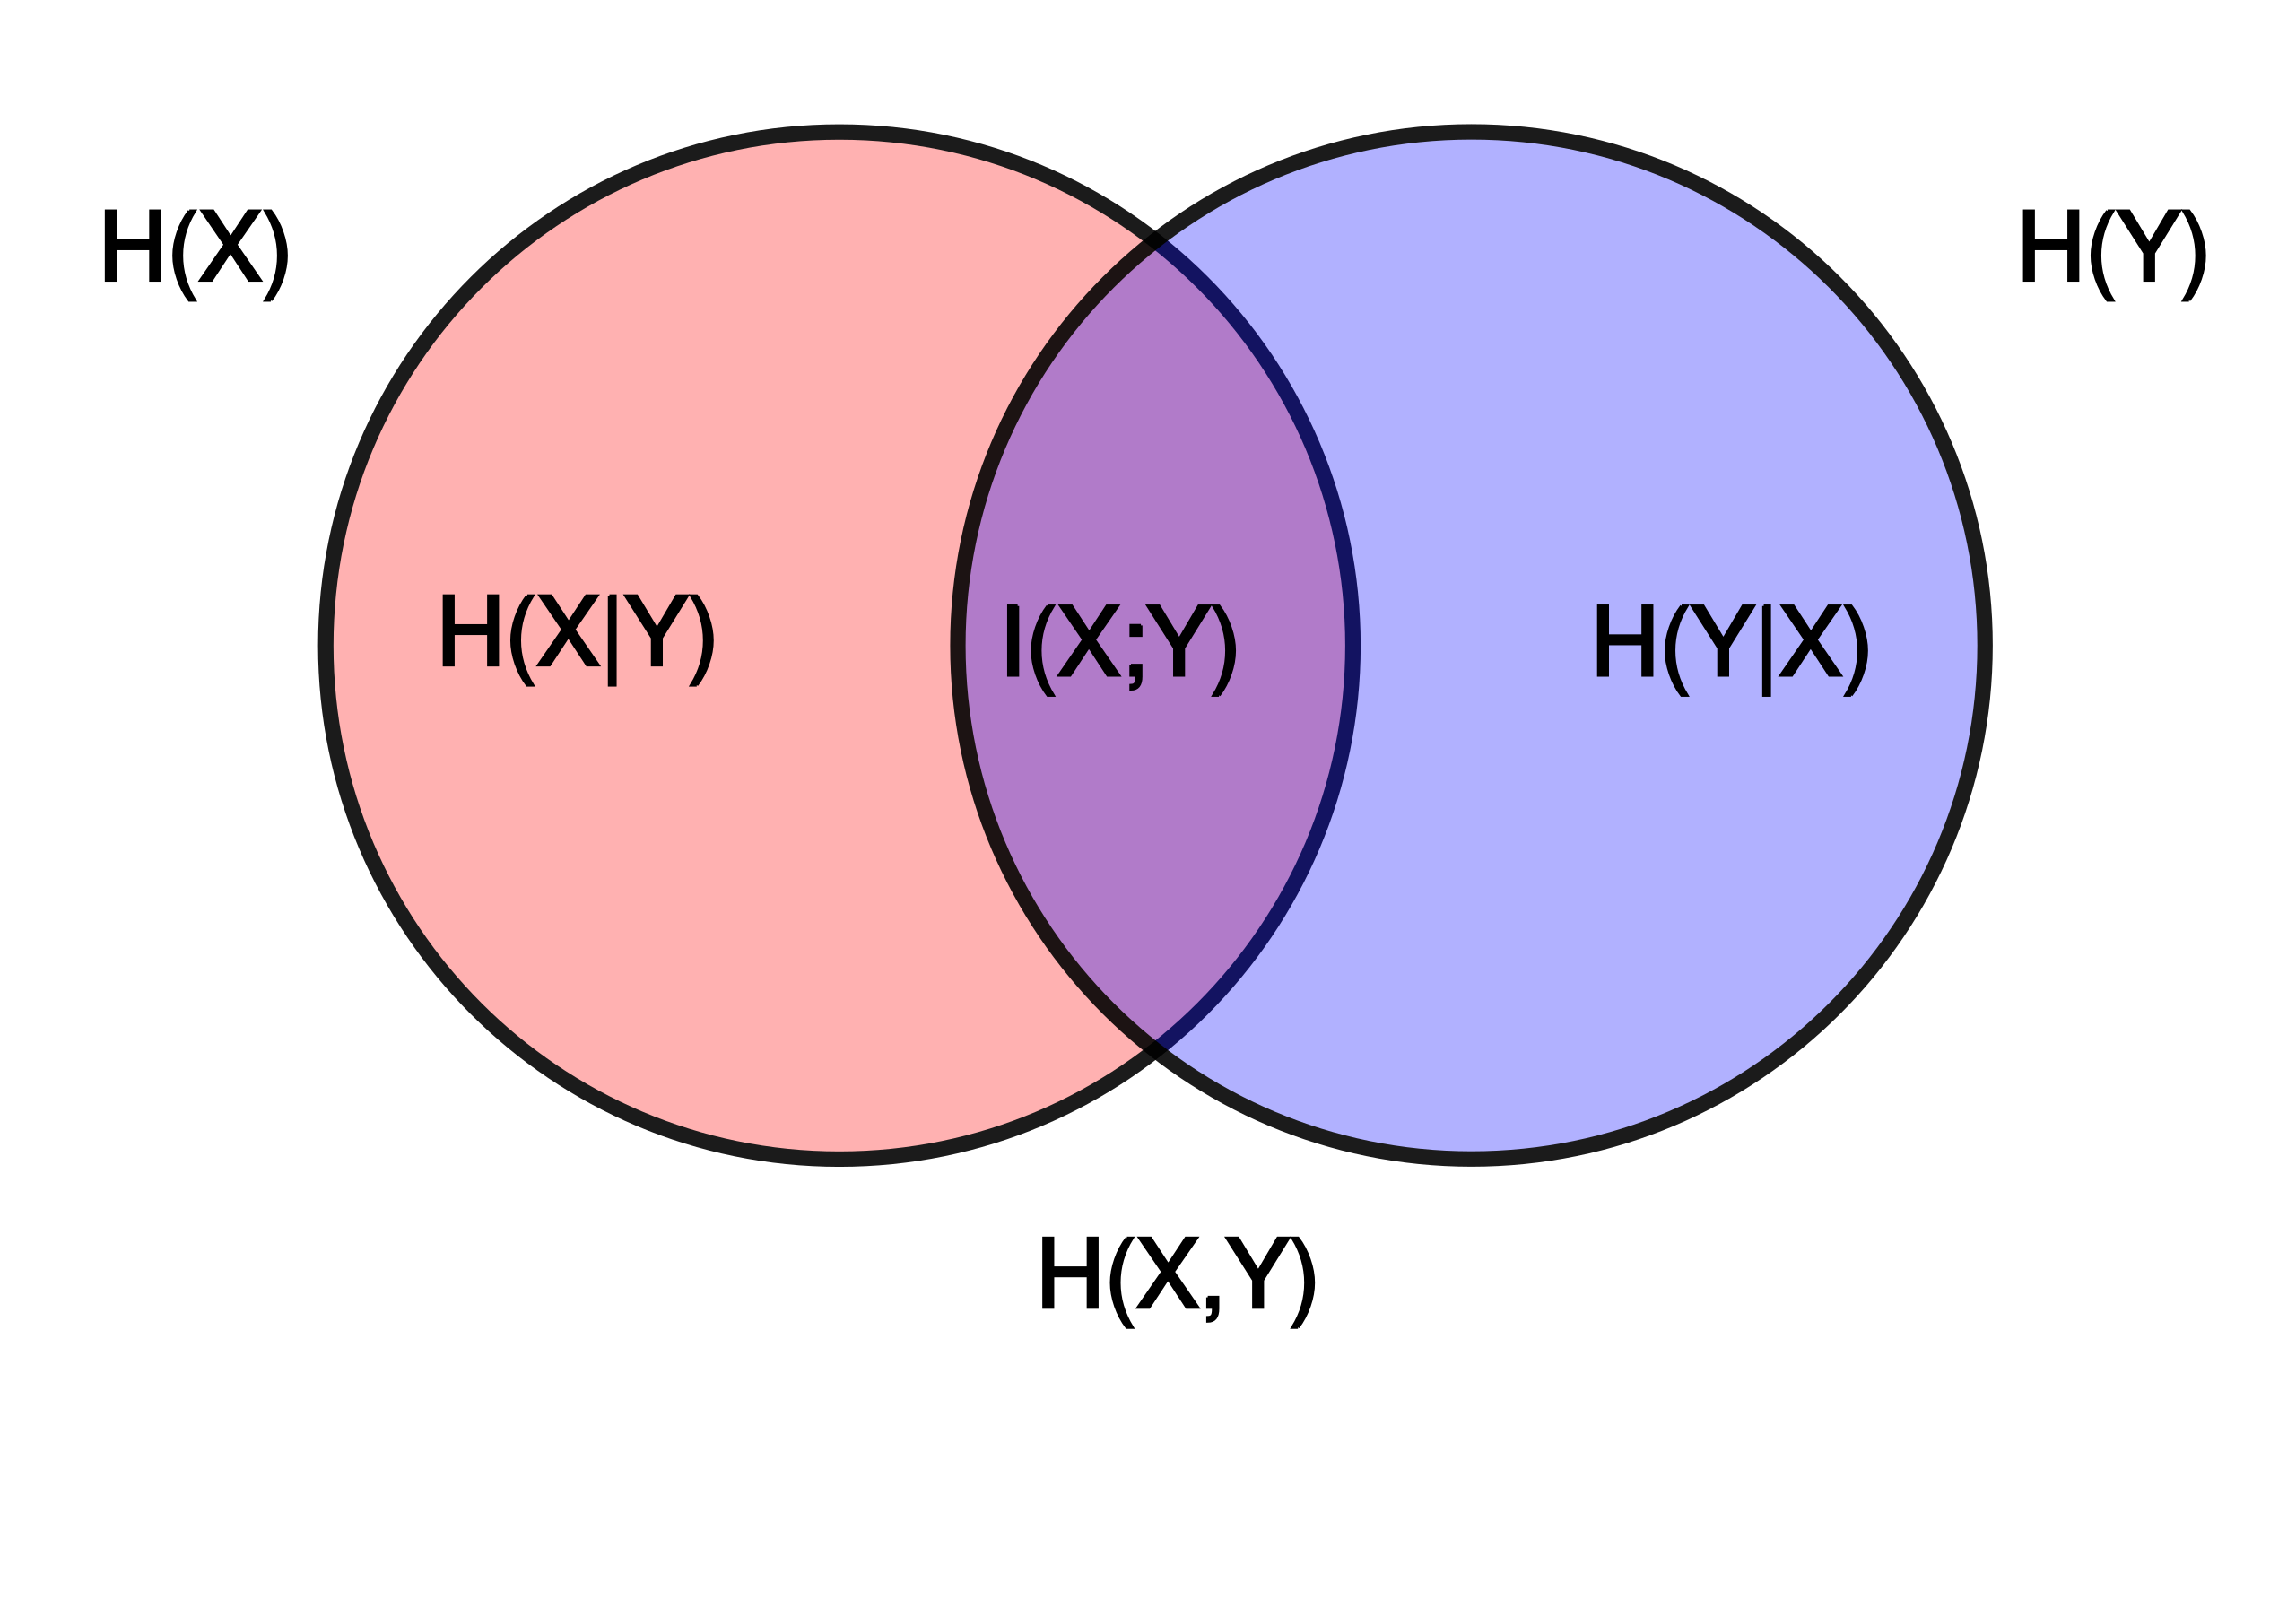
\includegraphics[width=\linewidth]{entropy-relation-diagram}
    \caption{Venn diagram showing additive and subtractive relationships various information measures associated with correlated variables X and Y}
  \end{figure}
  \column{0.6\textwidth}
  \begin{itemize}
    \item Entropy: $H(\pi) = - \sum^J_{j=1} \frac{|S_j|}{|N|} \log{\frac{|S_j|}{|N|}}$
    \item Conditional entropy: $H(\pi|\pi') = - \sum^J_{j=1} \sum^K_{k=1} \frac{|S_j \cap S'_k|}{|N|} \log{\frac{|S_j \cap S'_k|/|N|}{|S_k|/|N|}}$
    \item Mutual Information (MI): $\I(\pi, \pi') = H(\pi) - H(\pi|\pi')$
    \item Variation of Information (VI): $\VI(\pi, \pi') = H(\pi) + H(\pi') - 2\I(\pi, \pi')$, metric!
  \end{itemize}
  \end{columns}
\end{frame}

\begin{frame}{How different are two partitions, quantitatively?}{Baseline Values}
  \begin{columns}
  \column{0.5\textwidth}
  \begin{figure}
    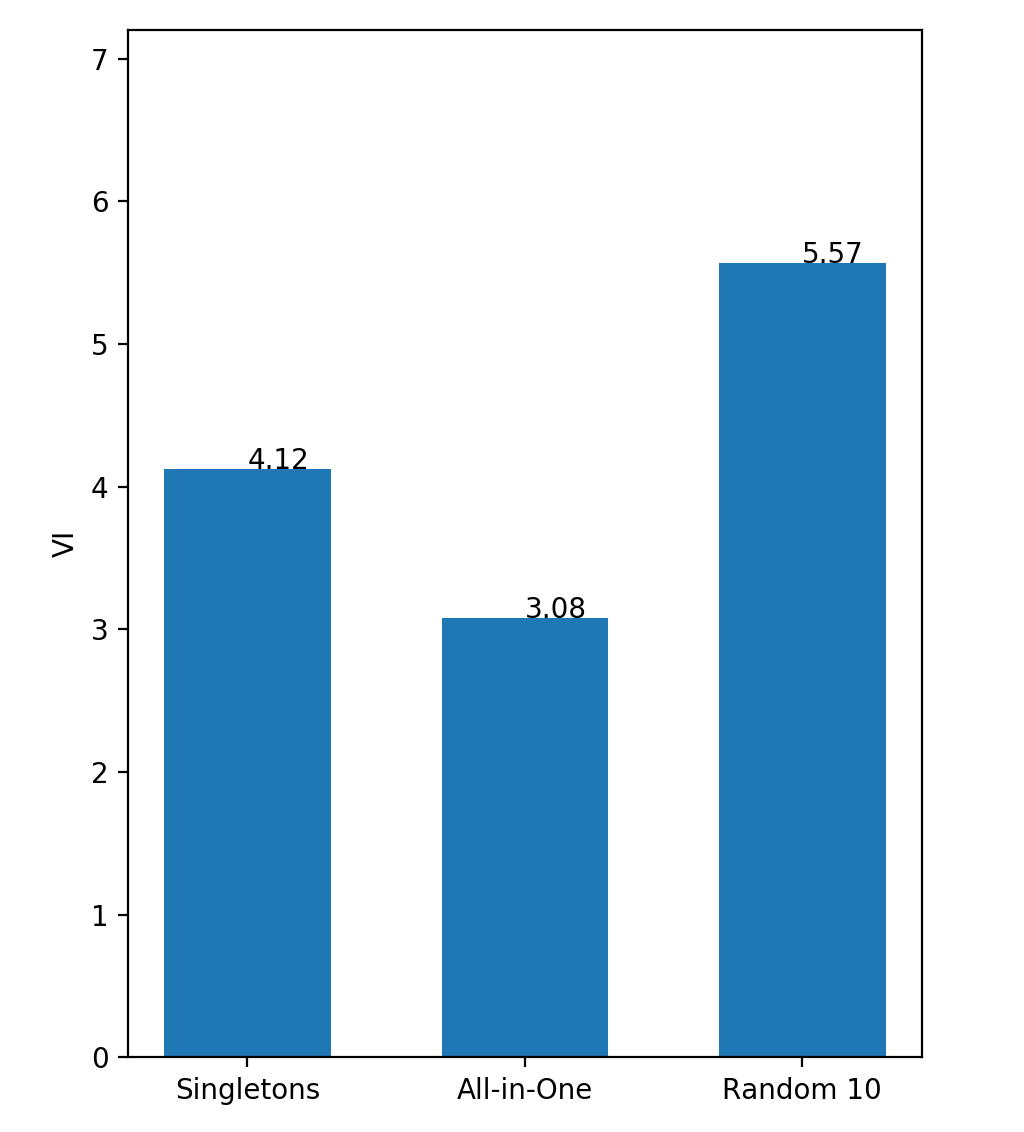
\includegraphics[width=\linewidth]{vi_baselines}
    \caption{The Knesset partition baseline VI values}
  \end{figure}
  \column{0.5\textwidth}
  \begin{figure}
    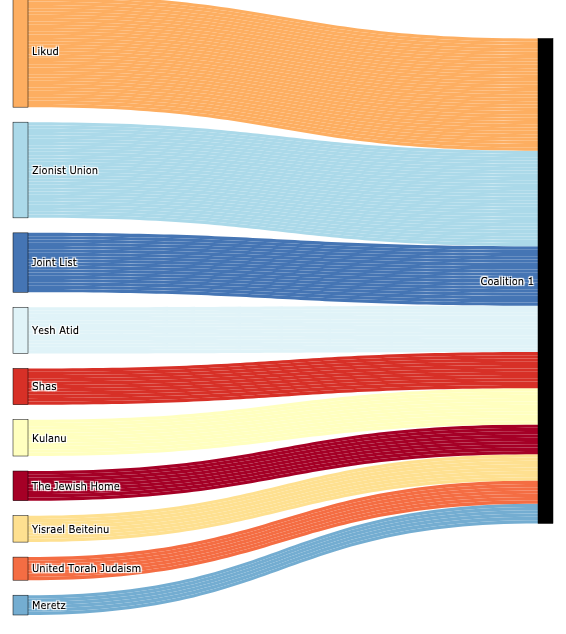
\includegraphics[width=\linewidth]{friends}
    \caption{All-in-One partition of the Knesset}
  \end{figure}
  \end{columns}
\end{frame}

\begin{frame}{How different are two partitions, quantitatively?}{Additional Measure: AMI}
  Adjusted Mutual Information (AMI):
  \[
    \AMI(\pi, \pi') = \frac{I(\pi, \pi') - E(I(\pi, \pi'))}{\max(H(\pi), H(\pi')) - E(I(\pi, \pi'))}
  \]
  \begin{itemize}
    \item Adjusted for chance
    \item Normalized: $\lbrack0, 1\rbrack$
    \item Not metric
  \end{itemize}

  Good for detecting ``bad'' (very different) partitions:
  \begin{table}[h]
  \centering
  \begin{tabular}{|c|c|}
  \hline
         & Ajusted Mutual Information \\ \hline
  Singletons & 3e-14 \\
  All-in-One & -5e-16 \\
  Randome 10 & 0.007 \\
  \hline
  \end{tabular}
  \caption{The Knesset partition baseline AMIs}
  \end{table}
\end{frame}

% You can reveal the parts of a slide one at a time
% with the \pause command:
\begin{frame}{Second Slide Title}
  \begin{itemize}
  \item {
    First item.
    \pause % The slide will pause after showing the first item
  }
  % You can also specify when the content should appear
  % by using <n->:
  \item<3-> {
    Third item.
  }
  % or you can use the \uncover command to reveal general
  % content (not just \items):
  \item<5-> {
    Fifth item. \uncover<6->{Extra text in the fifth item.}
  }
  \end{itemize}
\end{frame}

\begin{frame}{Main Theorem}
\begin{theorem}
Theorem Statements. Example for citation \cite{Author1990}.
\end{theorem}

\begin{proof}
Proof of the theorem goes here.
\end{proof}
\end{frame}

\section{Hedonic Game Stability Models}

\section{Machine Learning Models}

\section{Results \& Discussion}

\section{Conclusion}

\begin{frame}{Summary}
  \begin{itemize}
  \item
    The \alert{first main message} of your talk in one or two lines.
  \item
    The \alert{second main message} of your talk in one or two lines.
  \item
    Perhaps a \alert{third message}, but not more than that.
  \end{itemize}
  
  \begin{itemize}
  \item
    Outlook
    \begin{itemize}
    \item
      Something you haven't solved.
    \item
      Something else you haven't solved.
    \end{itemize}
  \end{itemize}
\end{frame}

% Placing a * after \section means it will not show in the
% outline or table of contents.
% Bibliography section. Use \bibitem to add more bibliography items.
\section*{Bibliography}
\begin{frame}{Bibliography}
  \begin{thebibliography}{10}

  \bibitem{Author1990}
    A.~Author.
    \newblock {\em Handbook of Everything}.
    \newblock Some Press, 1990.

  \bibitem{Someone2000}
    S.~Someone.
    \newblock On this and that.
    \newblock {\em Journal of This and That}, 2(1):50--100,
    2000.

  \end{thebibliography}
\end{frame}

\end{document}
